We promised that you would learn how to write everything you saw in the book. In this chapter, we continue exploring process networks, and learn how \tp is actually just two other processes stuck together with a channel.

\GOALS
Continue exploring process networks, as well as learn about \LEVELT and processes with multiple channel parameters.

\section{The Network}

\begin{figure}[h]
  \begin{center}
    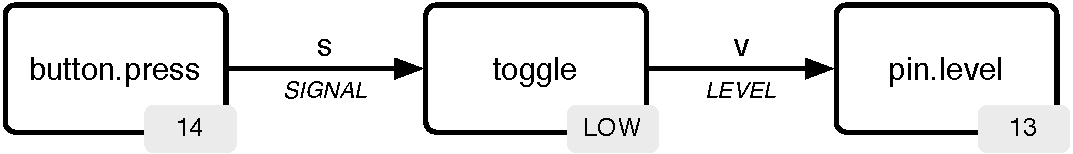
\includegraphics[width=\linewidth]{images/ch5-process-network}
    \caption{The process network for this chapter's code.}
    \label{diagram:ch5-process-network}
  \end{center}
\end{figure}

\CODE
\lstinputlisting[caption=Peeling away the layers of \tp.,label=code:inside-toggle]{code/inside-toggle.occ}

\section{The Circuit}
The circuit for this chapter is identical to Chapter~\ref{ch4}. You should be able to type in the code from this chapter, run it, and get exactly the same behavior as before. 

\PATTERNS
\plumbing programs are all about networks of processes sending information to each-other using channels. Channels are (we're sorry) the {\em plumbing} that makes our programs work. In the previous chapter, you saw how \bp sent a \SIGNALV to the process \tp, which then turned the built-in LED on and off. As it turns out, the process \tp is like a set of nesting Russian dolls: we can break it open, and find two more processes inside.

\subsection{Channels in, channels out}
Look at the process network (Figure~\vref{diagram:ch5-process-network}) once more. From this network, we can see that the \bp process still sends a \SIGNALV when we press the button. Now, instead of communicating with a  process named \tp, we instead send a \SIGNALV to a process called \toggle. 

If you focus your attention on \toggle only (Figure~\vref{diagram:ch5-just-toggle}), you'll see that it has one channel coming in from the left, and one channel going out on the right. The \toggle process waits until it receives a \SIGNALV on the channel {\code s}; when it does, it sends out a message on the channel {\code v}. 

\begin{figure}[h]
  \begin{center}
    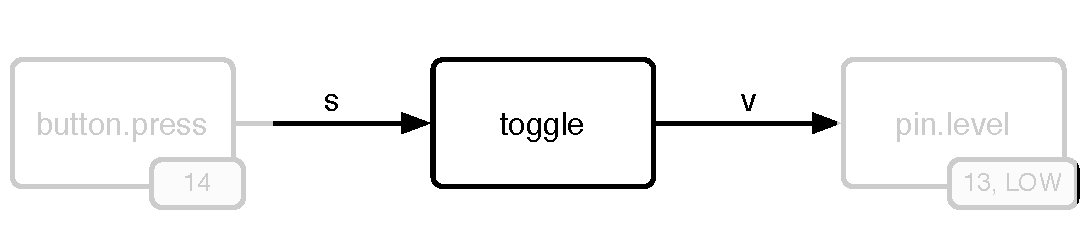
\includegraphics[width=\linewidth]{images/ch5-just-toggle}
    \caption{Toggle has one channel in, and one channel out.}
    \label{diagram:ch5-just-toggle}
  \end{center}
\end{figure}

If the diagram has a process that has one channel in and one channel out, that means the code must as well. There is a strong link between the process networks we draw and the code we write when we're working in \plumbing. If you look at line 7, you'll see that the process \toggle has two parameters. One is the receiving end of the channel {\code s?}, and the other is the sending end of the channel {\code v!}. This matches the channels in our diagram: the channel labeled {\code s} is drawn as going from \bp to \toggle, and the channel labeled {\code v} is drawn from \toggle to \pl.

\subsection{Declaring Multiple Channels}
For every arrow (channel) in our process network, we need to declare a channel in our code. In the last chapter, we saw a process network with two processes and one channel. In this chapter, we have three processes and two channels. (There's no trickery here: I'm counting boxes (processes) and arrows (channels) in the process network diagram. It really is that easy.) If you look at lines 2 and 3 of the code, you'll see that the two channels are not the same. We'll pull lines 2 and 3 out so they are easier to focus on:

\begin{lstlisting}[firstnumber=2]
  CHAN SIGNAL s:
  CHAN LEVEL  v:
\end{lstlisting}
	
	Line 2 says that {\code s} is a channel that has a particular shape. We would say it carries information of type \SIGNALT. Line 3 says that {\code v} is a channel that has a {\em different} shape. It carries a different {\em type} of information. Instead of carrying a \SIGNALV, it instead carries \LEVELT messages. Whereas a signal is like a submarine ping, a \LEVELT is either \HIGH or \LOW.
	
In the last chapter, we said that the communication between two processes was like a high-five (Figure~\vref{diagram:high-five-channel-comms}). {\strong This is still true.} However, when the high-five happens, a note on a piece of paper is passed along from one process to the next. In this case, because the channel carries notes of type \LEVELT, that note either has the value \HIGH or \LOW written on it.

% This is the first good use of "pattern". Perhaps the other section should be called "About the Code".
\section{Pattern: A Pipeline}
A pipeline carries stuff from one place to another. When we string multiple processes together in a straight line, we have constructed a {\strong pipeline} of processes. It is, essentially, an assembly line, where each process processes some information, and then passes the result of that work along. In \plumbing, each process has to wait for information from the ``upstream'' process; that is, \pl waits for messages (a high-five) from \toggle, and \toggle waits for messages from \bp. In technical terms, this would be called a {\em buffered, synchronous} pipeline.\webnote{http://en.wikipedia.org/wiki/Pipeline_(computing)}{pipelines in computing}. 

The Pipeline is one of the simplest patterns for processing information in parallel. It shows up everywhere, from the command-line on Linux, to the way a web server handles requests from your web browser, to the central processing unit in your computer. The Pipeline is one of the Big Ideas in computing.

Congratulations. You've just explored it on your Arduino.

\EXPLORATIONS
You can explore a number of things at this point. 

\begin{description}
	\item[\il]\ \\
	There are many processes in the \plumbing library; one you haven't seen yet is called \il. It takes in a \LEVELT value on one channel and outputs the opposite value on another. That is, it has a \LEVELT channel coming in, and a \LEVELT channel going out. Try using it in your process network---it only fits in one place.
	\item[\tick]\ \\
	The \tick process has one channel coming out of it that carries messages of type \SIGNALT. It generates a \SIGNALV on a fixed schedule, over and over, like the ticking of a clock. To generate a \SIGNALV once every second (or once every 1000ms), you would write
	\begin{verbatim}
		tick(ch!, 1000)
	\end{verbatim}
	This assumes, of course, that you had properly declared a channel called {\code ch!}. You can replace one of the processes in the code for this chapter with a \tick process. Can you figure out which process can be replaced?
\end{description}

\BREAKAGE
It may seem like we come up with lots of ways to break your code at the end of every chapter. That's because we want you to experience as many errors as possible in a controlled way before we set you free.

\begin{description}
	\item[Wrong channel types]\ \\
	What happens if you take the code we started with and swap around \SIGNALT and \LEVELT on lines 2 and 3? Do things still work?
	\item[Wrong channel order]\ \\
	Modify line 7 so that \toggle has its read and write channels in the wrong order. That is, flip it from {\code (s?, v!)} to {\code (v!, s?)}.
	\item[Wrong channel directions]\ \\
		Modify line 7 so that \toggle has its read and write channels are pointing in the wrong direction. That is, flip it from {\code (s?, v!)} to {\code (s!, v?)}. (Subtle, no? Don't worry. If you draw pictures first, this is a difficult mistake to make.)
  \item[Wrong pin number]\ \\
	What happens if you have the wrong pin number in either \bp or \pl?
	\item[Initial state flip]\ \\
	What happens if you change \pl so that it starts with \HIGH instead of \LOW?
	\item[Forgetting a process]\ \\
	What happens if you simply remove \toggle? (Draw a new version of the process network from this chapter, and leave out \toggle. Does that look right? This is what happens when you remove line 7 from your program!)
\end{description}	
	
	

